윤수는 스타링크 노래 맞히기를 좋아한다. 스타링크 노래 맞히기는 주어진 노래를 듣고 먼저 제목을 맞히는 사람이 점수를 얻는 게임이다. 절대 음감을 가진 윤수는 노래의 첫 네 음만 듣고도 어떤 노래든 바로 맞출 수 있다. 정환은 윤수랑 맞서 싸울 수 있는 프로그램을 만들려고 한다. 다음은 TwinkleTwinkleLittleStar(반짝반짝 작은 별)의 악보 중 일부이다.
\begin{center}
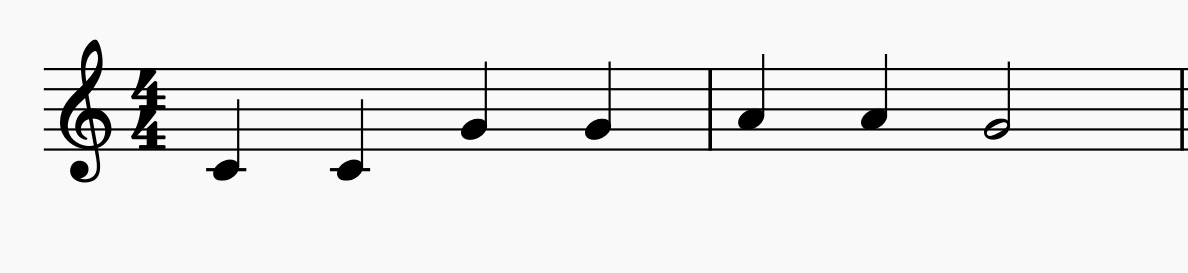
\includegraphics[bb=0 0 100 200]{starlink.png}
\end{center} 

악보를 박자와 관계없이 음이름으로 표현하면 다음과 같다. "CCGGAAG"[도도솔솔라라솔]

윤수를 이기기 위해서는 이 프로그램이 첫 세 음인 CCG만 듣고 노래 제목인 TwinkleTwinkleLittleStar를 출력할 수 있어야 한다. 세상의 모든 노래를 아는 윤수와 다르게 정환은 음을 아는 노래가 $N$개 뿐이다. 만약 노래의 첫 음 3개로 시작하는 노래가 여러개 있어 무슨 노래인지 알 수 없는 경우 \t{?}를 출력한다. 또한, 정환이 알지 못하는 노래가 나올 경우 \t{!}를 출력한다.

정환을 도와서 첫 세 음만 듣고 본인이 음을 아는 노래를 맞추는 프로그램을 완성시키자. 이 프로그램은 대문자와 소문자를 구분한다.
